Unlike the previous chapters here we only require experience, and not a complete knowledge of the env.
The term \textit{Monte Carlo} is often used in a more broad sense for any estimation method that
invlolves a significant random component.
We are learning the value function based on the sample returns from the MDP.
The idea of gaining experience and averaging returns from each state to estimate the value functions
is an essential idea of all MC methods.
In comparison to DP algorithms, that are breadth-first we can view MCMs as depth-first
algorithms.
MCMs do not bootstrap - an estimation of the value of one state is not based on estimations
of value functions for other states.

\section{Monte Carlo Prediction}
\textit{First-visit MC methods} average returns following the first visit to state $s$.
\textit{Every-visit MC methods} average returns following every visit to state $s$.
\begin{center}
    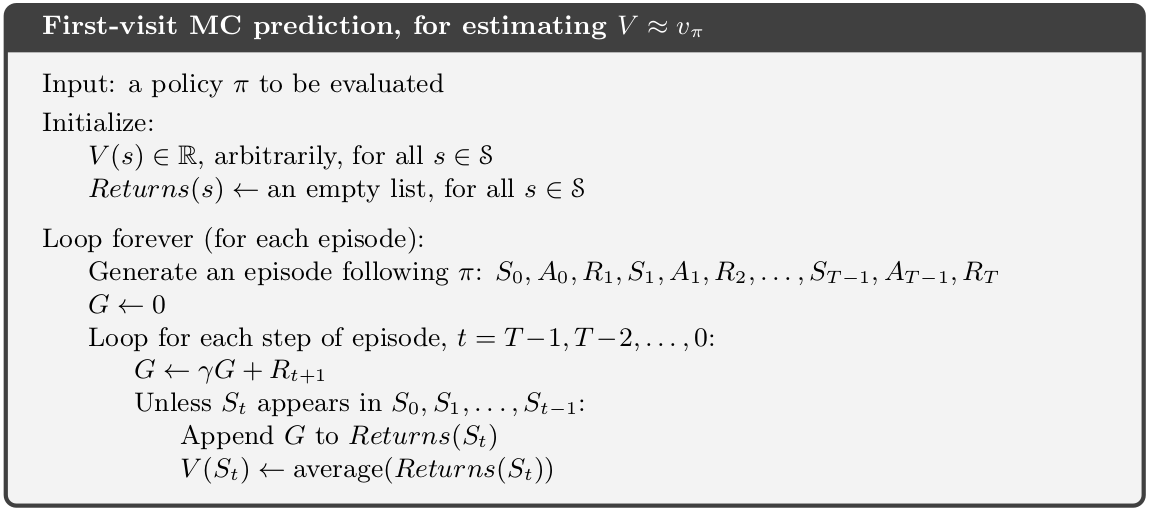
\includegraphics[width=\textwidth]{img/first_visit_MCM.png}
\end{center}

\section{Monte Carlo Estimation of Action Values}
The problem of lack of exploration.
Possible solution with exploring starts, even though this can be used only under specific
circumstances.

\section{Monte Carlo Control}
\begin{center}
    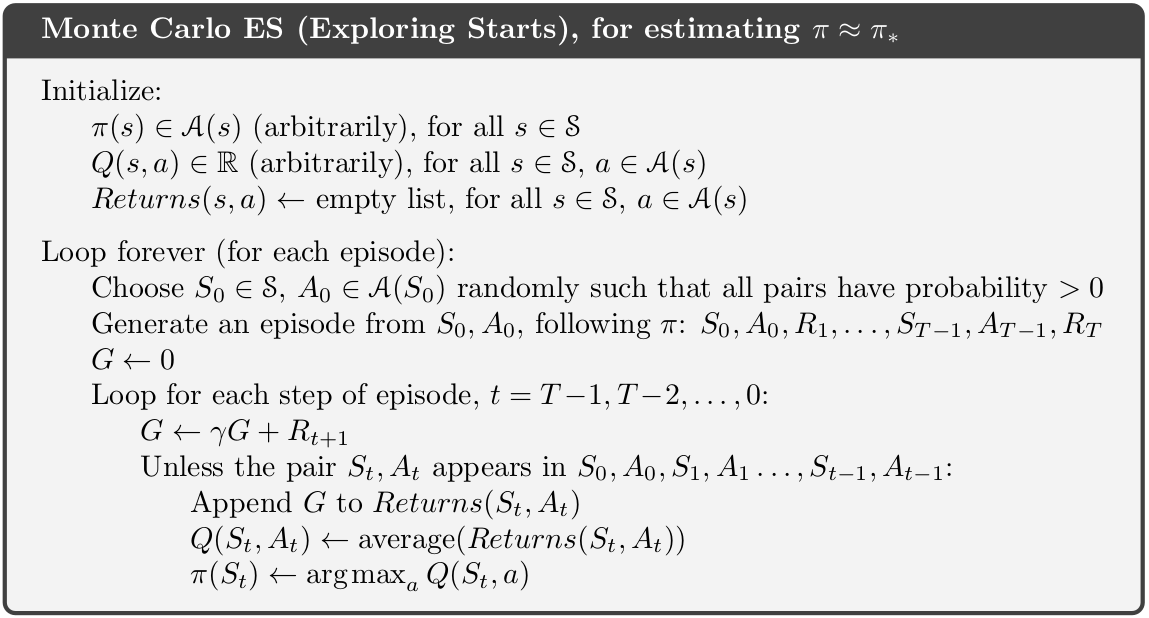
\includegraphics[width=\textwidth]{img/alg_MCM_ES.png}
\end{center}
We can modify the algorithm to only store the mean and the count in $Returns$, rather than the whole list
of returns.
This way we optimize in memory consumption and remove the time needed to calculate the average when
storing $Q(S_t, A_t)$.

\section{Monte Carlo Control without Exploring Starts}
\emph{On-policy methods}\label{t:on_policy_methods} evaluate or improve the policy used to
make decisions, whereas \emph{off-policy methods}\label{t:off_policy_methods} evaluate or
improve a policy different from the one used to make decisions.
\begin{center}
    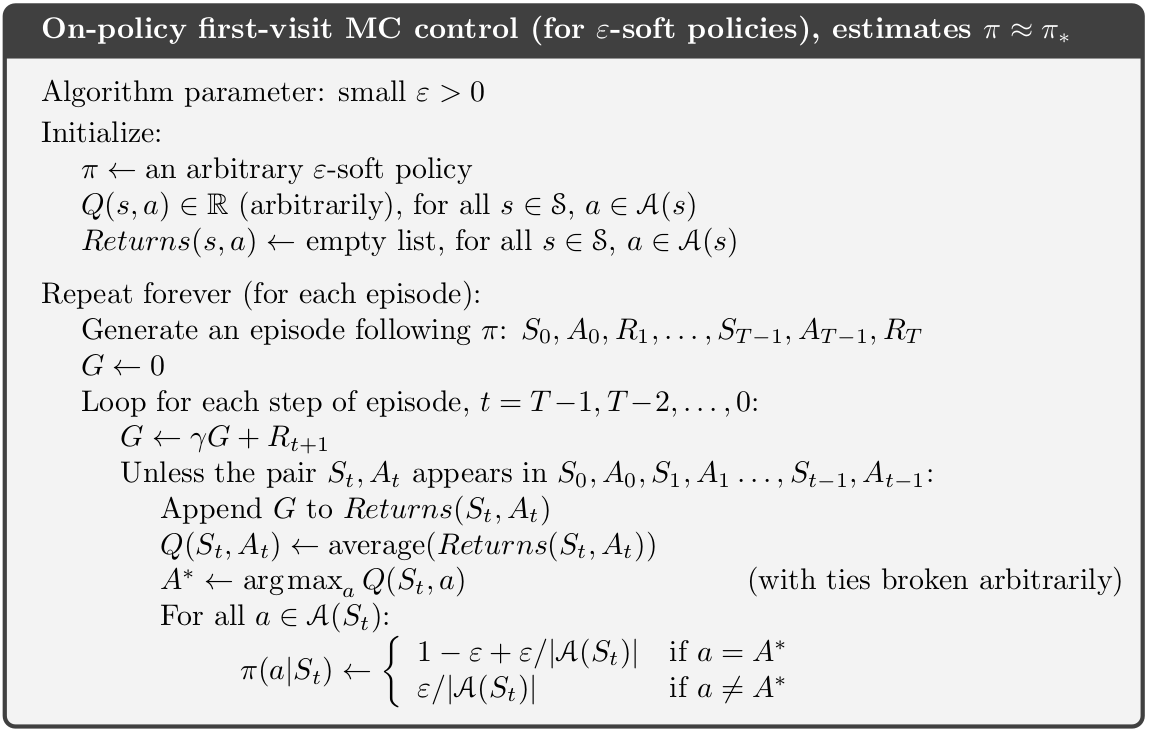
\includegraphics[width=\textwidth]{img/alg_on_policy_first_visit_MC_control.png}
\end{center}

\section{Off-policy Prediction via Importance\newline Sampling}
\label{sec:off_policy_prediction_via_importance_sampling}
Learn the optimal policy while behaving according to an exploratory policy.
The policy being learned about is the \textit{target policy}, and the policy used to generate
behavior is called the \textit{behavior policy}.
\textit{Off-policy} methods are usually of greater variance and slower to converge.
If $b$ is the behavior policy and $\pi$ the target policy then
$\pi(a\mid s)>0\rightarrow b(a\mid s)>0$ - this is called the assumption of \textit{coverage}.
Meaning that every state, action for which $\pi$ has a non-zero value (covers it), policy
$b$ also has a non-zero value, and technically will eventually cover it too.
\newline\emph{Importance sampling ratio}\label{t:importance_sampling_ratio} given a
state-action trajectory:
\begin{myequation}{5.3}
    \rho_{t:T-1}\doteq \prod_{k=t}^{T-1}\frac{\pi(A_k\mid S_k)}{b(A_k\mid S_k)}
\end{myequation}
We use the importance sampling ratio to transform the estimated $v_b(s)$ to $v_\pi(s)$:
\begin{myequation}{5.4}
    v_{\pi}(s) = \mathbb{E}\left[\rho_{t:T-1}\cdot G_t\mid S=s\right]
\end{myequation}
Here the timesteps will surpass episode boundaries.
If we define $\mathcal{T}(s)$ as a set of all time steps where $s$ was encountered;
only the first times per episode for first-visit methods.
Let $T(t)$ denote the first time of termination after $t$, and $G_t$ denote the return after $t$ following
up to $T(t)$, then we can estimate $v_\pi(s)$ as:
\begin{myequation}{5.5}
    V(s)\doteq\frac{\sum_{t\in\mathcal{T}(s)}\rho_{t:T(t)-1}G_t}{|\mathcal{T}(s)|}
\end{myequation}
When \emph{importance sampling} is done as a simple average in this way it's called
\emph{ordinary importance sampling}\label{t:ordinary_importance_sampling}.
An important alternative to that is
\emph{weighted importance sampling}\label{t:weighted_importance_sampling} that uses
weighted averages:
\begin{myequation}{5.6}
    V(s)\doteq\frac{\sum_{t\in\mathcal{T}(s)}\rho_{t:T(t)-1}G_t}
    {\sum_{t\in\mathcal{T}(s)}\rho_{t:T(t)-1}}
\end{myequation}

\section{Incremental Implementation}
\begin{center}
    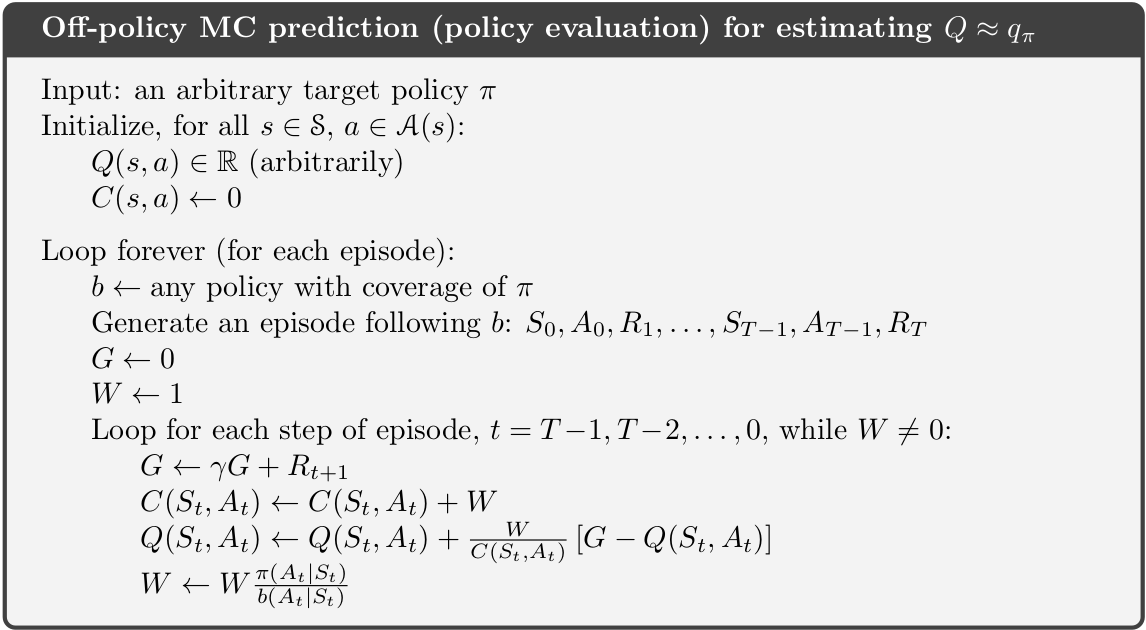
\includegraphics[width=\textwidth]{img/alg_off_policy_mc_prediction.png}
    \begin{itemize*}
        \item $C(s,a)$: cumulative sum of the weights.
    \end{itemize*}
\end{center}

\section{Off-policy Monte Carlo Control}
\begin{center}
    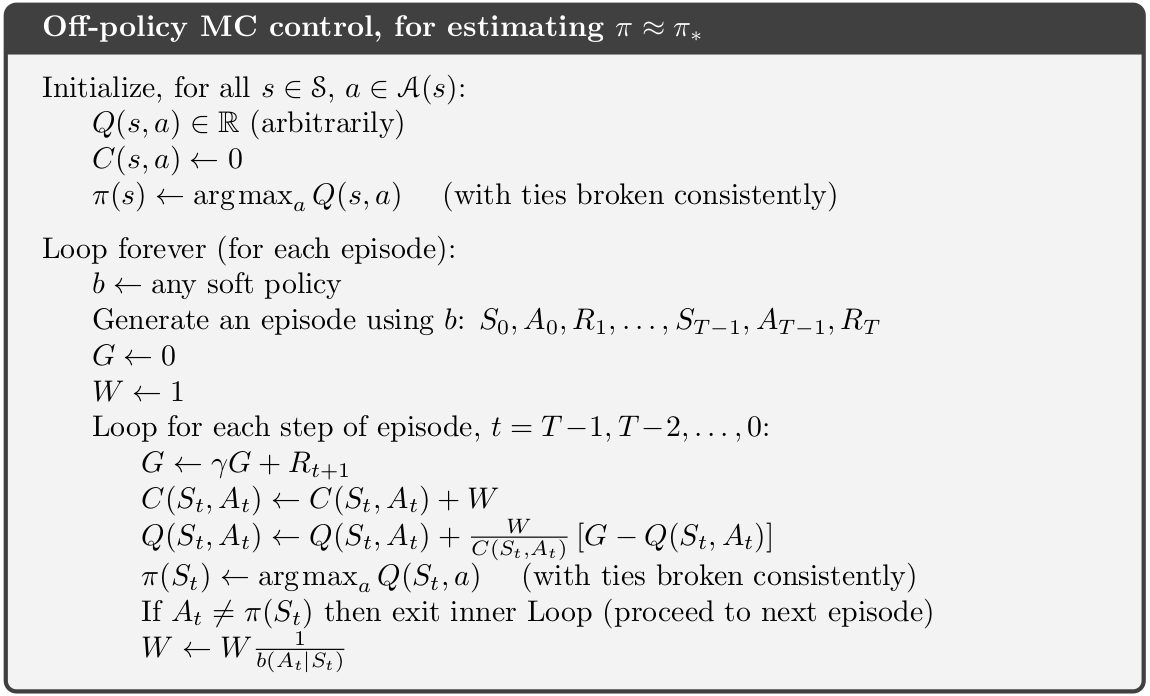
\includegraphics[width=\textwidth]{img/alg_off_policy_mc_control.png}
\end{center}

\section{*Discounting-aware Importance Sampling}
\emph{Importance sampling} ($\rho$) takes into account all timesteps leading up to $T$.
What it should preferably be doing is looking at the discount to $G$ which is $\gamma$ and
using that to discount the $\rho$.
We can look into $\gamma$ as partially terminating $G$ and then define
\emph{flat partial returns} ($\bar{G}_{t:h}$) as:

\begin{equation*}
    \bar{G} \doteq R_{t+1} + R_{t+2} + \cdots + R_h,
    \hspace{3em}
    0 \leq t \le h \leq T
\end{equation*}

They're called \emph{flat} because there's no discounting, and \emph{partial} because rather
than going to $T$ they end at $h$, called the \emph{horizon}.

\begin{equation*}
    G_t \doteq (1-\gamma)\sum_{h=t+1}^{T-1}\gamma^{h-t-1}\bar{G}_{t:h}
        + \gamma^{T-t-1}\bar{G}_{t:T}
\end{equation*}

Given this, (\ref{eq:5.5}) and (\ref{eq:5.6}) become discount aware importance
sampling estimators:

\begin{myequation}{5.9}
    V(s)\doteq\frac{
        \sum_{t\in\mathcal{T}(s)}\left(
            (1-\gamma)\sum_{h=t+1}^{T(t)-1}\gamma^{h-t-1}\rho_{t:h-1}\bar{G}_{t:h}+
            \gamma^{T(t)-t-1}\rho_{t:T(t)-1}\bar{G}_{t:T(t)}
        \right)
    }{|\mathcal{T}(s)|}
\end{myequation}

\begin{myequation}{5.10}
    V(s)\doteq\frac{
        \sum_{t\in\mathcal{T}(s)}\left(
            (1-\gamma)\sum_{h=t+1}^{T(t)-1}\gamma^{h-t-1}\rho_{t:h-1}\bar{G}_{t:h}+
            \gamma^{T(t)-t-1}\rho_{t:T(t)-1}\bar{G}_{t:T(t)}
        \right)
    }{
        \sum_{t\in\mathcal{T}(s)}\left(
            (1-\gamma)\sum_{h=t+1}^{T(t)-1}\gamma^{h-t-1}\rho_{t:h-1}+
            \gamma^{T(t)-t-1}\rho_{t:T(t)-1}
        \right)
    }
\end{myequation}

\section{*Per-decision Importance Sampling}
\label{sec:per_decision_importance_sampling}
To further minimize the variance, we can multiply a given $R$ at time $t$ with just the
$\rho_{t0:t-1}$ because those after do not influence the reward.

\begin{equation*}
    \begin{gathered}
        \mathbb{E}\left[\rho_{t:T-1}R_{t+k}\right]=\mathbb{E}\left[\rho_{t:t-k-1}R_{t+k}\right]
        \Rightarrow
        \mathbb{E}\left[\rho_{t:T-1}G_t\right]=\mathbb{E}\left[\tilde{G}_t\right] \\
        \tilde{G}_t=\rho_{t:t}R_{t+1}+\gamma\rho_{t:t+1}R_{t+2}+\cdots
        +\gamma^{k-1}\rho_{t:t+k-1}R_{t+k}+\cdots+\gamma^{T-1}\rho_{t:T-1}R_T\\
    \end{gathered}
\end{equation*}

Now (\ref{eq:5.5}) becomes:

\begin{myequation}{5.15}
    V(s)=\frac{\sum_{t\in\mathcal{T}(s)}\tilde{G}_t}{|\mathcal{T}(s)|}
\end{myequation}

\section{Summary}
The Monte Carlo methods presented in this chapter learn value functions and optimal
policies from experience in the form of sample episodes.
This gives them at least three kinds of advantages over DP methods.
\begin{enumerate}
    \item They can be used to learn optimal behavior directly from interaction with the
    environment, with no model of the environment’s dynamics.
    \item They can be used with simulation or sample models.
    For surprisingly many applications it is easy to simulate sample episodes even though
    it is difficult to construct the kind of explicit model of transition probabilities
    required by DP methods.
    \item It is easy and efficient to focus Monte Carlo methods on a small subset of the states.
    A region of special interest can be accurately evaluated without going to the expense of
    accurately evaluating the rest of the state set (we explore this further in Chapter 8).
    \item They may be less harmed by violations of the Markov property.
    This is because they do not update their value estimates on the basis of the value
    estimates of successor states.
    In other words, it is because they do not bootstrap.
\end{enumerate}

In designing Monte Carlo control methods we have followed the overall schema of
\myref{sec:gpi}{GPI} introduced in Chapter 4.
\myref{sec:gpi}{GPI} involves interacting processes of
\myref{sec:policy_evaluation}{policy evaluation} and
\myref{sec:policy_improvement}{policy improvement}.
Monte Carlo methods provide an alternative \myref{sec:policy_evaluation}{policy evaluation}
process.
Rather than use a model to compute the value of each state, they simply average many returns
that start in the state.
Because a state’s value is the expected return, this average can become a good approximation
to the value.
In control methods we are particularly interested in approximating action-value functions,
because these can be used to improve the policy without requiring a model of the
environment’s transition dynamics.
Monte Carlo methods intermix policy evaluation and policy improvement steps on an
episode-by-episode basis, and can be incrementally implemented on an episode-by-episode basis.
Maintaining sufficient exploration is an issue in Monte Carlo control methods.
It is not enough just to select the actions currently estimated to be best, because then no
returns will be obtained for alternative actions, and it may never be learned that they
are actually better.
One approach is to ignore this problem by assuming that episodes begin with state–action pairs
randomly selected to cover all possibilities.
Such \emph{exploring starts} can sometimes be arranged in applications with simulated episodes,
but are unlikely in learning from real experience.
In \myref{t:on_policy_methods}{on-policy methods}, the agent commits to always exploring and tries to find the
best policy that still explores.
In \myref{t:off_policy_methods}{off-policy methods}, the agent also explores, but learns a deterministic optimal policy that
may be unrelated to the policy followed.
\emph{Off-policy prediction} refers to learning the value function of a target policy from data
generated by a different behavior policy.
Such learning methods are based on some form of
\myref{sec:off_policy_prediction_via_importance_sampling}{importance sampling}, that is,
on weighting returns by the ratio of the probabilities of taking the observed actions under
the two policies, thereby transforming their expectations from the behavior policy to the
target policy.
\myref{t:ordinary_importance_sampling}{Ordinary importance sampling} uses a simple average of
the weighted returns, whereas
\myref{t:weighted_importance_sampling}{weighted importance sampling} uses a weighted average.
Ordinary importance sampling produces unbiased estimates, but has larger, possibly infinite,
variance, whereas weighted importance sampling always has finite variance and is preferred in
practice.
Despite their conceptual simplicity, \myref{t:off_policy_methods}{off-policy}
Monte Carlo methods for both prediction and control remain unsettled and are a subject
of ongoing research.
The Monte Carlo methods treated in this chapter differ from the DP methods treated
in the previous chapter in two major ways.
\begin{enumerate}
    \item They operate on sample experience, and thus can be used for direct learning
    without a model.
    \item They do not bootstrap.
    That is, they do not update their value estimates on the basis of other value estimates.
\end{enumerate}
These two differences are not tightly linked, and can be separated.
In the next chapter we consider methods that learn from experience, like Monte Carlo methods,
but also bootstrap, like DP methods.
